% Created by tikzDevice version 0.12.3.1 on 2022-09-01 12:20:23
% !TEX encoding = UTF-8 Unicode
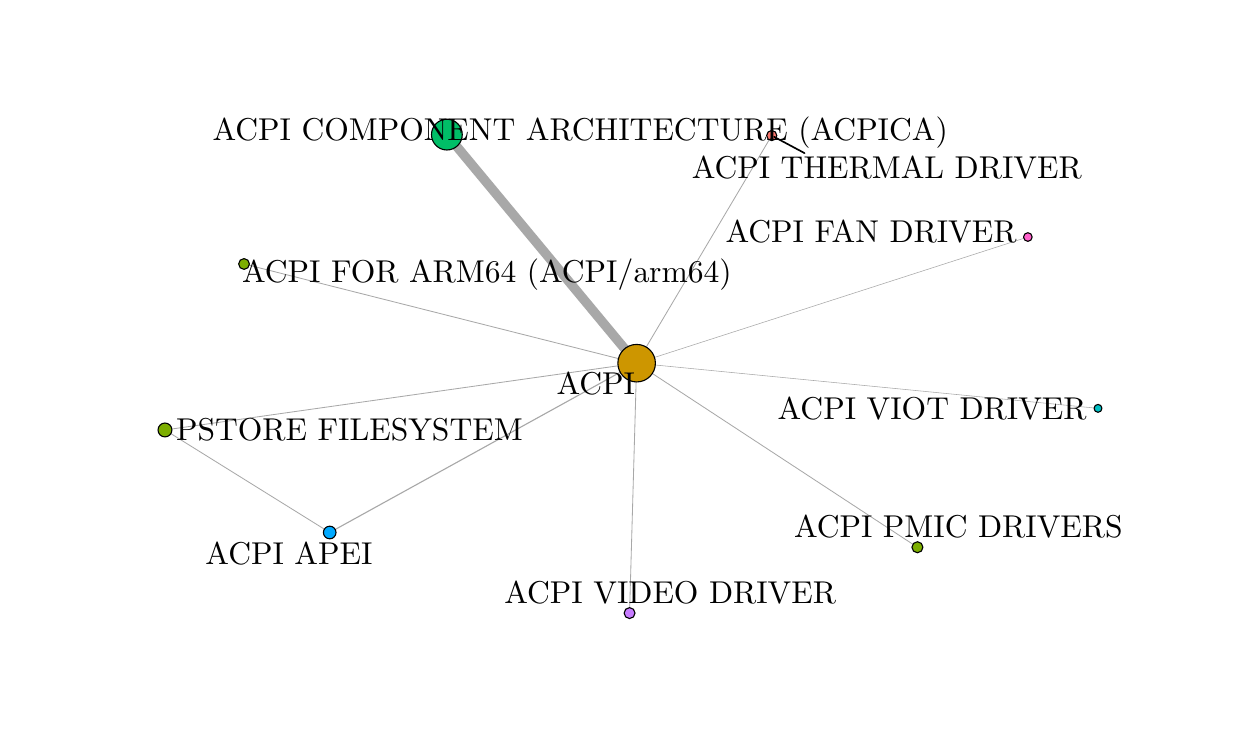
\begin{tikzpicture}[x=1pt,y=1pt]
\definecolor{fillColor}{RGB}{255,255,255}
\path[use as bounding box,fill=fillColor,fill opacity=0.00] (0,0) rectangle (433.62,252.94);
\begin{scope}
\path[clip] (  0.00,  0.00) rectangle (433.62,252.94);
\definecolor{fillColor}{RGB}{255,255,255}

\path[fill=fillColor] (  0.00,  0.00) rectangle (433.62,252.94);
\end{scope}
\begin{scope}
\path[clip] ( 32.75, 32.75) rectangle (403.62,222.94);
\definecolor{drawColor}{gray}{0.66}

\path[draw=drawColor,line width= 0.4pt,line join=round] (220.05,131.70) -- (109.14, 70.52);

\path[draw=drawColor,line width= 3.4pt,line join=round] (220.05,131.70) -- (151.48,214.30);

\path[draw=drawColor,line width= 0.2pt,line join=round] (220.05,131.70) -- (361.41,177.29);

\path[draw=drawColor,line width= 0.3pt,line join=round] (220.05,131.70) -- ( 78.18,167.55);

\path[draw=drawColor,line width= 0.3pt,line join=round] (220.05,131.70) -- (321.51, 65.19);

\path[draw=drawColor,line width= 0.3pt,line join=round] (220.05,131.70) -- (268.86,213.95);

\path[draw=drawColor,line width= 0.3pt,line join=round] (220.05,131.70) -- (217.49, 41.40);

\path[draw=drawColor,line width= 0.2pt,line join=round] (220.05,131.70) -- (386.76,115.38);

\path[draw=drawColor,line width= 0.3pt,line join=round] (220.05,131.70) -- ( 49.61,107.57);

\path[draw=drawColor,line width= 0.3pt,line join=round] (109.14, 70.52) -- ( 49.61,107.57);
\definecolor{drawColor}{RGB}{0,0,0}
\definecolor{fillColor}{RGB}{205,150,0}

\path[draw=drawColor,line width= 0.4pt,line join=round,line cap=round,fill=fillColor] (220.05,131.70) circle (  6.78);
\definecolor{fillColor}{RGB}{0,169,255}

\path[draw=drawColor,line width= 0.4pt,line join=round,line cap=round,fill=fillColor] (109.14, 70.52) circle (  2.28);
\definecolor{fillColor}{RGB}{0,190,103}

\path[draw=drawColor,line width= 0.4pt,line join=round,line cap=round,fill=fillColor] (151.48,214.30) circle (  5.56);
\definecolor{fillColor}{RGB}{255,97,204}

\path[draw=drawColor,line width= 0.4pt,line join=round,line cap=round,fill=fillColor] (361.41,177.29) circle (  1.56);
\definecolor{fillColor}{RGB}{124,174,0}

\path[draw=drawColor,line width= 0.4pt,line join=round,line cap=round,fill=fillColor] ( 78.18,167.55) circle (  1.95);

\path[draw=drawColor,line width= 0.4pt,line join=round,line cap=round,fill=fillColor] (321.51, 65.19) circle (  1.99);
\definecolor{fillColor}{RGB}{248,118,109}

\path[draw=drawColor,line width= 0.4pt,line join=round,line cap=round,fill=fillColor] (268.86,213.95) circle (  1.84);
\definecolor{fillColor}{RGB}{199,124,255}

\path[draw=drawColor,line width= 0.4pt,line join=round,line cap=round,fill=fillColor] (217.49, 41.40) circle (  1.97);
\definecolor{fillColor}{RGB}{0,191,196}

\path[draw=drawColor,line width= 0.4pt,line join=round,line cap=round,fill=fillColor] (386.76,115.38) circle (  1.43);
\definecolor{fillColor}{RGB}{124,174,0}

\path[draw=drawColor,line width= 0.4pt,line join=round,line cap=round,fill=fillColor] ( 49.61,107.57) circle (  2.51);

\path[draw=drawColor,line width= 0.6pt,line join=round,line cap=round] (280.73,207.60) -- (269.72,213.49);

\node[text=drawColor,anchor=base,inner sep=0pt, outer sep=0pt, scale=  1.14] at (205.28,120.21) {ACPI};

\node[text=drawColor,anchor=base,inner sep=0pt, outer sep=0pt, scale=  1.14] at ( 94.41, 59.05) {ACPI APEI};

\node[text=drawColor,anchor=base,inner sep=0pt, outer sep=0pt, scale=  1.14] at (199.66,212.10) {ACPI COMPONENT ARCHITECTURE (ACPICA)};

\node[text=drawColor,anchor=base,inner sep=0pt, outer sep=0pt, scale=  1.14] at (304.77,175.46) {ACPI FAN DRIVER};

\node[text=drawColor,anchor=base,inner sep=0pt, outer sep=0pt, scale=  1.14] at (165.92,160.87) {ACPI FOR ARM64 (ACPI/arm64)};

\node[text=drawColor,anchor=base,inner sep=0pt, outer sep=0pt, scale=  1.14] at (336.29, 68.86) {ACPI PMIC DRIVERS};

\node[text=drawColor,anchor=base,inner sep=0pt, outer sep=0pt, scale=  1.14] at (310.43,198.26) {ACPI THERMAL DRIVER};

\node[text=drawColor,anchor=base,inner sep=0pt, outer sep=0pt, scale=  1.14] at (232.19, 45.02) {ACPI VIDEO DRIVER};

\node[text=drawColor,anchor=base,inner sep=0pt, outer sep=0pt, scale=  1.14] at (326.84,111.46) {ACPI VIOT DRIVER};

\node[text=drawColor,anchor=base,inner sep=0pt, outer sep=0pt, scale=  1.14] at (116.25,103.65) {PSTORE FILESYSTEM};
\end{scope}
\end{tikzpicture}
